\section{Lambert's problem}

In the context of astrodynamics and orbital mechanics, Lambert's problem is the
boundary value problem (BVP) in the context of the restricted two-body problem
dynamics. Equation \ref{eq:lambert-bvp} models this problem.

\begin{equation}
    \ddot{\vec{r}} = -\frac{\mu}{r^3}\vec{r} \quad \begin{cases}
        \vec{r}(t_1) = \vec{r}_1 \\ 
        \vec{r}(t_2) = \vec{r}_2 \\ 
        \Delta t = t_2 - t_1
    \end{cases}
    \label{eq:lambert-bvp}
\end{equation}

Figure \ref{fig:lambert-geometry} depicts the geometry of the problem. If the
initial position vector $\vec{r}_1$ is the position of the Earth at time $t_1$
and vector $\vec{r}_2$ is the position of an interloper at time $t_2$, then it
is possible to find the targeting orbit required to transfer a spacecraft
between the two.

The solution to the Lambert's problem returns the values of $\vec{v_1}$ and
$\vec{v_2}$, which complete the targeting orbit state vectors at launch and
arrival positions.

Solving Lambert's problem requires numerical routines. Lots of algorithms have
been devised over the last century. The author of this document some of the most
popular ones and compared them in performance, see \cite{martinez2021}.

\begin{figure}[H]
    \centering
    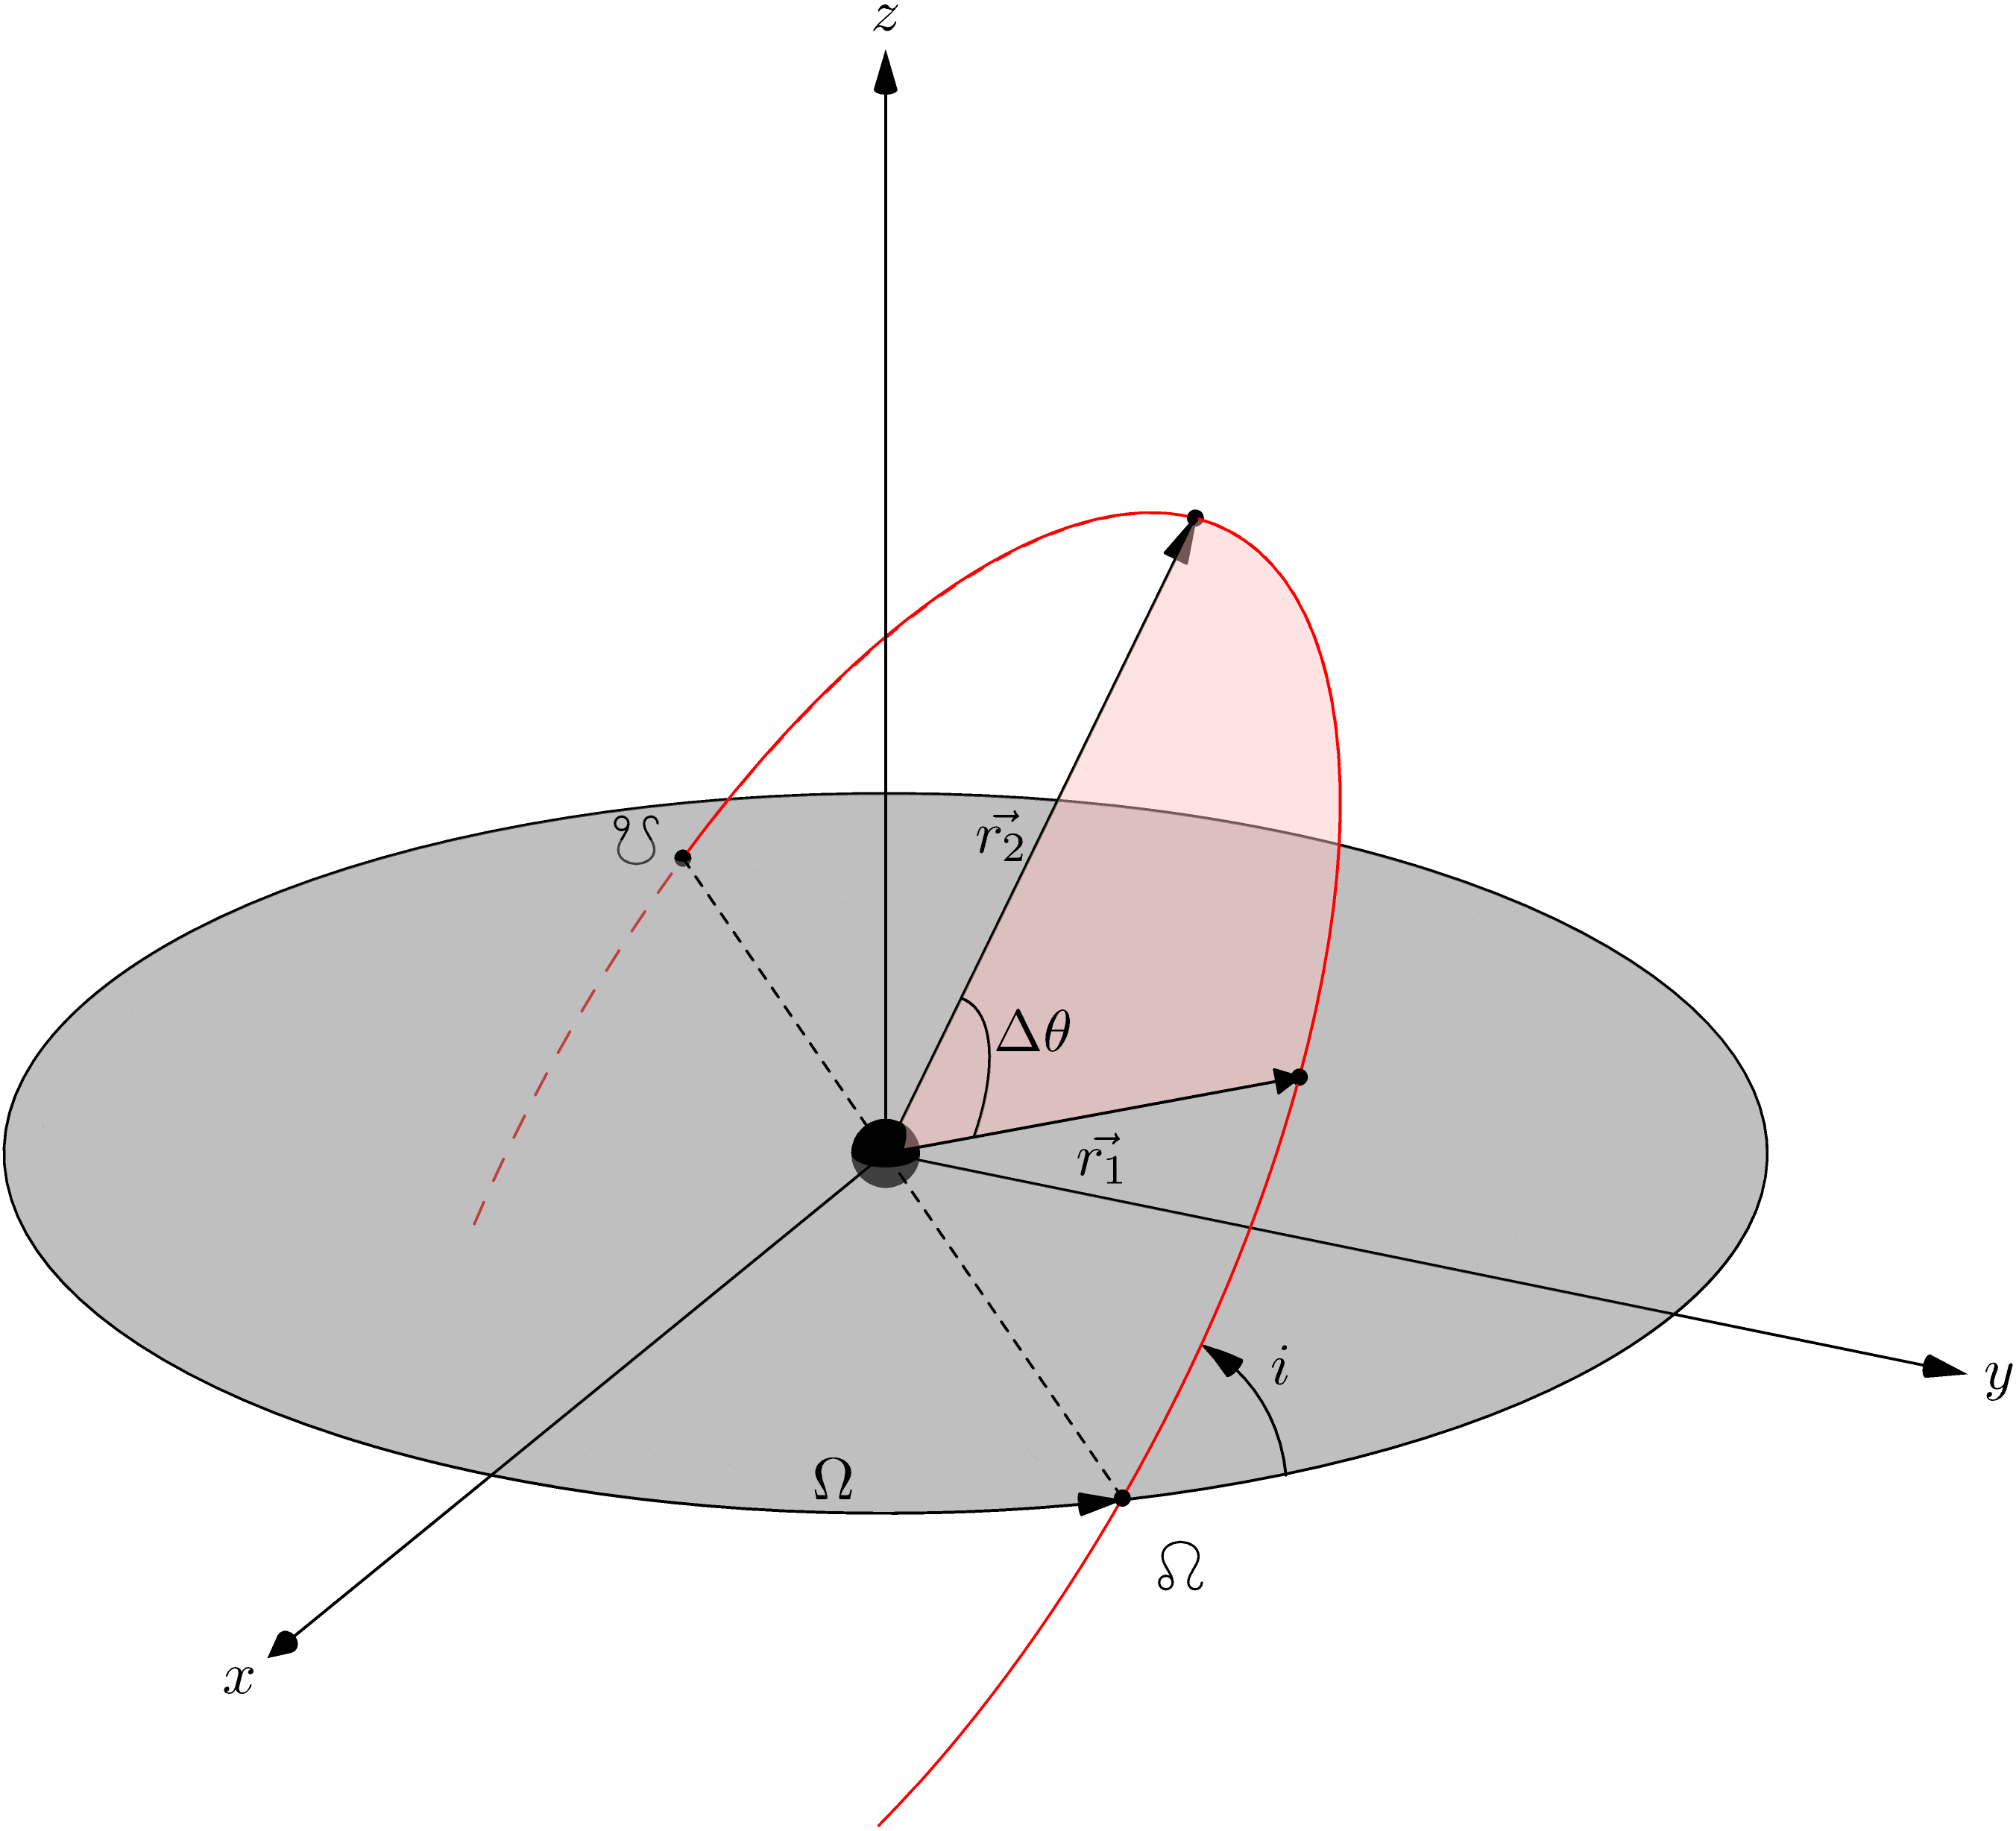
\includegraphics[width=0.75\textwidth]{lambert-problem/geometry.png}
    \caption{Lambert's problem geometry. The targeting orbit is represented by the red curve.}
    \label{fig:lambert-geometry}
\end{figure}

Once solved, the modulus of the velocities can be used to compute for the
required $\Delta v$. This is the increment in the velocity that needs to be
achieved by the propulsion system in order to insert the spacecraft into the
desired targeting orbit.

The $\Delta v$ relates with the characteristic energy $C_3$, also known as
specific energy. Equation \ref{eq:c3} summarizes this relation for hyperbolic
orbits:

\begin{equation}
        C_3 = v_{\infty}^2
        \label{eq:c3}
\end{equation}
